\documentclass[letterpaper, 10 pt, conference]{ieeeconf} 

\IEEEoverridecommandlockouts                             
\overrideIEEEmargins

\usepackage[english]{babel}
\usepackage[T1]{fontenc}
\usepackage{amsmath}
\usepackage{graphicx}

\title{\LARGE \bf Distributed Machine Learning Technology in Edge-cloud Environment: A Survey }
\author{Weiwei Wu$^{1}$ and Lin Wang$^{2}$}

\begin{document}
\maketitle
\thispagestyle{empty}
\pagestyle{empty}
\selectlanguage{english}
\begin{abstract}
Resource-constrained IoT devices, such as sensors and actuators, have become ubiquitous in recent years. This has led to the generation of large quantities of data in real-time, which is an appealing target for AI systems. However, deploying machine learning models on such end-devices is nearly impossible. A typical solution involves offloading data to external computing systems (such as cloud servers) for further processing but this worsens latency, leads to increased communication costs, and adds to privacy concerns. To address this issue, efforts have been made to place additional computing devices at the edge of the network, i.e close to the IoT devices where the data is generated. Deploying machine learning systems on such edge computing devices alleviates the above issues by allowing computations to be performed close to the data sources. This survey describes major research efforts where machine learning systems have been deployed at the edge of computer networks, focusing on the operational aspects including compression techniques, tools, frameworks, and hardware used in successful applications of intelligent edge systems.
\end{abstract}
\begin{keywords}
edge intelligence, edge computing, machine learning, low-power, deep learning, distributed computing, edge-cloud.
\end{keywords}

\section{Introduction}
Due to the explosive growth of wireless communication technology, the number of Internet of Things (IoT) devices has increased dramatically in recent years. It has been estimated that by 2020, more than 25 billion devices will have been connected to the Internet\cite{mahdavinejad_machine_2018}. IoT devices typically have limited computing power and small memories. Examples of such resource constrained IoT devices include sensors, microphones, smart fridges, and smart lights. IoT devices and sensors continuously generate large amounts of data, which is of critical importance to many modern technological applications such as autonomous vehicles.

One of the best ways to extract information and make decisions from this data is to feed those data to a machine learning (ML) system. Unfortunately, limitations in the computational capabilities of resource-constrained devices inhibit the deployment of ML algorithms on them. So, the data is offloaded to remote computational infrastructure, most commonly cloud servers, where computations are performed. Transferring raw data to cloud servers increases communication costs, causes delayed system response, and makes any private data vulnerable to compromise. To address these issues, it is natural to consider processing data closer to its sources and transmitting only the necessary data to remote servers for further processing \cite{chen_editorial_2013}.

\section{Distributed Training}
Distributed training of DL models on multiple edge-devices and/or the cloud has two significant benefits:
\begin{itemize}
	\item Data acquired from end-devices can be used for training/re-training at the edge-servers, thereby reducing the communication overhead of transmitting to and training on a central cloud server.
	\item It also leads to greater privacy since no central location has access to data produced by end-devices.
\end{itemize}
The next two sections discuss collaborative and privacy-aware learning on the end-edge-cloud architecture
\subsection{Algorithms based on gradient descent}
For distributed training for algorithms based on gradient descent. Wang et al. introduced a technique to train ML models at the edge without the help of external computation systems such as cloud servers \cite{wang_when_2018}. They focused on algorithms that use gradient-based approaches for training (including SVMs, K-means, linear regression and convolution neural networks (CNNs) ). Their technique minimizes the loss function of a learning model by using the computational power of edge-devices only.

Local gradient descent is performed on multiple edge-devices based on data received at each device (i.e. on local datasets). This produces locally updated copies of the ML model. These copies are sent to another edge-device, known as the aggregator, that computes a weighted average of all the locally updated models. This averaged model is sent back to all the edge-devices so that each device now carries a model averaged over training data from all edge-devices.

The next iteration performs local updates once again and the process repeats until resource consumption reaches a prespecified budget.
To demonstrate the effectiveness of this technique, three Raspberry Pi devices and a laptop computer were used as edge-devices. They were connected via WiFi to an additional laptop computer that was used as the aggregator. Three datasets (viz., MNIST, Facebook metrics, and User Knowledge Modeling) were used to evaluate the ML models. The technique's performance was close to the optimum for training different ML models on different datasets.
\subsection{Federated learning}
Federated Learning (FL) is a family of distributed ML methods that involve collaborative training of shared prediction DNN models on devices such as mobile phones\cite{McMahan_Moore_Ramage_Hampson_Arcas_2017}. All training data is kept on the end-devices and model training occurs in powerful local or cloud computing infrastructure. In general, there are two steps in the FL training process, viz. i) local training and ii) global aggregation. In local training, the end-device downloads the model from a central cloud server, computes an updated model using that local data to improve model performance. After that, an encrypted communication service is used to send a summary of all updates made by the end-device to the server. The server aggregates these updated models (typically by averaging) to construct an improved global model, as illustrated in Figure 1. This decentralized ML approach ensures the maximum use of available end-devices and does not share any data among end-devices, which helps to enhance the security and privacy of the local data. However, federated learning faces challenges that include communication overhead, interoperability of heterogeneous devices, and resource allocation\cite{Li_Sahu_Talwalkar_Smith_2020, Lim_Luong_Hoang_Jiao_Liang_Yang_Niyato_Miao_2020}.
\begin{figure}[bh] 
	\centerline{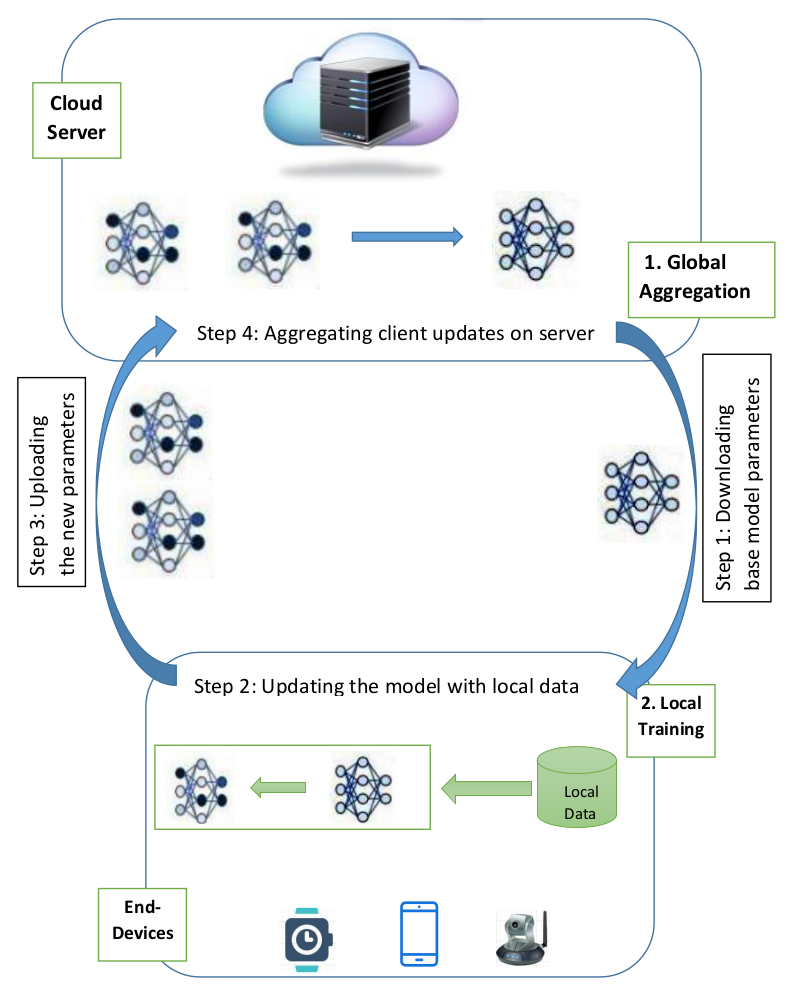
\includegraphics[width=8cm]{FederatedLearning.png}}
	\vspace*{8pt}
	\caption{Federated learning allows training on end-devices where the data is produced. First, end-devices download parameters of a trainable ML model from the cloud server. Then, those devices update the model locally with their own data. After that, all end-devices upload the updated model parameters. Finally, the cloud server aggregates multiple client updates to improve the model.}
\end{figure}
Federated learning with heterogeneous edge clients can lead to slow learning when some edge clients have very low-resources. To address this problem, Nishio and Yonetani introduce FedCS which performs federated learning with an intelligent client selection mechanism to ensure faster learning of high performing ML models \cite{Nishio_Yonetani_2018}.

Exchanging model parameters and other data between edge-devices and cloud servers is mandatory for training an edge-cloud-based DL model. However, as the size of the training model increases, more data needs to be exchanged between edge-devices and cloud servers. The high network communication cost is a bottleneck training a model. Various techniques have been proposed to reduce communication costs during training:
\begin{itemize}
	\item Lui et al. introduced intermediate edge aggregation before FL server aggregation \cite{Liu_Zhang_Song_Letaief_2019}.
	\item Wang et al. compare each client's local model update with the global update of the model at a central server. If the local update differs significantly from the global update, it is not communicated to the central server since it will become less relevant when updates are aggregated \cite{WANG_WANG_LI_2019}.
	\item Tao and Li introduced a new method called Edge Stochastic Gradient Descent (eSGD)\cite{Tao_Li_2018} that is capable of reducing the gradient size of a CNN model by up to 90\% by communicating only the most important gradients. On MNIST, they obtained an accuracy of 91.22\% with a 50\% gradient drop.
	\item Lin et al. studied the effect of gradient exchange in distributed stochastic gradient descent (DSGD) and found 99.9\% of gradient exchanges to be redundant\cite{Lin_Han_Mao_Wang_Dally_2020}. This observation inspired them to propose deep gradient compression, which compress the gradient from 270 to 600 times without losing much accuracy. They applied momentum correction, local gradient clipping, momentum factor masking, and warm-up training methods to reduce the size of gradient updates for training ResNet-50 from 97 MB to 0.35 MB, and for training DeepSpeech\cite{Hannun_Case_Casper_Catanzaro_Diamos_Elsen_Prenger_Satheesh_Sengupta_Coates_et} from 488 MB to 0.74 MB.
\end{itemize}
\subsection{Privacy in learning}
Privacy of sensitive training data becomes an issue when training is performed in a distributed fashion. Techniques derived from cryptography can be applied for hiding updates of local devices from a central aggregation server\cite{Bonawitz_Ivanov_Kreuter_Marcedone_McMahan_Patel_Ramage_Segal_Seth_2017} and also for hiding the aggregated update from the local devices\cite{Geyer_Klein_Nabi_2018}. While ensuring such local and global privacy mechanism, it is important to i) contain any drop in accuracy ii) ensure low overheads of computation and communication and iii) introduce robustness to communication errors and delays.

Mao et al. presented a privacy-aware DNN training architecture that uses differential privacy to protect user data during the training\cite{Mao_Yi_Li_Feng_Xu_Zhong_2018}. This deep learning scheme is capable of training a model using multiple mobile devices and the cloud server collaboratively, with minimal additional cost. First, this algorithm selects one convolutional layer to partition the neural network into two parts. One part runs on edge-devices, while another part runs on the server (AWS cloud server). The first part takes raw data with sensitive user information as input and uses a differentiable private activation algorithm to generate the volume of activations as output. These output activations contain Gaussian noise, which prevents external cloud servers from reproducing original input information using reversing activations. These noisy output activations are then transmitted to cloud servers for further processes. The servers take output activations as input and run the subsequent training process. This model was evaluated using a Nexus 6P phone and AWS based servers. The authors report that they have achieved good accuracy by deploying this model on Labeled Faces in the Wild dataset (LFW).

In order to avoid centralized aggregation of potentially sensitive information, block-chains have been explored as an alternative\cite{Kim_Moon_2018}. However, the compute power and energy requirements of mining on edge-devices remains an important challenge\cite{Wang_Han_Leung_Niyato_Yan_Chen_2020}.

\section{Distributed deep learnings inference}
Distributed deep neural network architectures allow the distribution of deep neural networks (DNNs) on the edge-cloud infrastructure in order to facilitate local and fast inference on edge-devices wherever possible. The success of a distributed neural network model depends on keeping inter-device communication costs as low as possible. Several attempts have been made to split and distribute a model between edge-devices, resulting in faster inference. DNN inference can be distributed in two ways, a) vertically, along the end-edge-cloud architecture, and b) horizontally, along multiple devices at the same level in the architecture.
\begin{figure}[bh] 
	\centerline{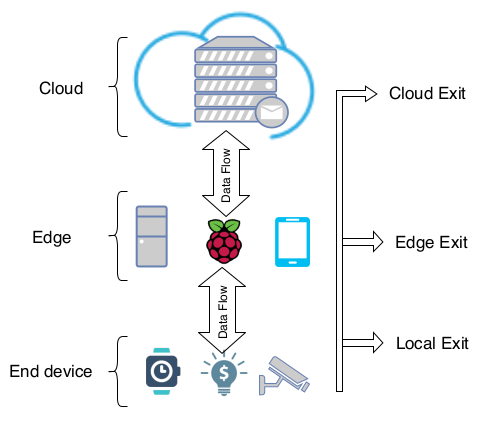
\includegraphics[width=8cm]{DDNN-Tee.png}}
	\vspace*{8pt}
	\caption{A high-level view of the distributed deep neural network (DDNN) approach designed by Teerapittayanon et al.\cite{Teerapittayanon_McDanel_Kung_2017}. End-devices send summary information to a local aggregator which serves as a DNN layer. The DDNN is jointly trained with all resource-constrained end-devices and exit points, so the network is capable of automatically collecting and combining input data from different end-devices. If the information collected from a particular end-device is sufficient to classify a sample then classification is done locally (i.e. on the end-device itself). Otherwise, the information is sent to the edge-servers for further processing. If edge-servers can complete the classification, they send the result back to the end-devices. Otherwise, edge-servers send the information to the cloud, where the classification process is completed, and the results returned to the end-devices.}
\end{figure}
\subsection{Vertically-distributed inference}
We now describe two orthogonal approaches for exploiting the vertical direction of the end-edge-cloud architecture. In the first approach mobile deep inference (MODI), the dynamic status of the architecture is considered to make optimal decisions about which model to run and where to run it. In the second approach Early exit of inference (EEoI), resources along the vertical direction are exploited to exit as early as possible in order to make optimal inferences while balancing the trade-off between accuracy on the one hand and computational effort and latency on the other.

\textbf{Mobile Deep Inference (MODI) Platform.} Due to variable network conditions, inference on the end-edge-cloud architecture is a dynamic problem. Static ap-proaches such as on-device inference only or remote inference only are both sub-optimal. Ogden and Guo\cite{Ogden_Guo_2018} propose a dynamic solution to this problem by designing a distributed platform for mobile deep inference. They propose to store multiple DL models (compressed and uncompressed) in a centralized model manager and dynamically deciding which model to run on which device based on the inference environment (memory, bandwidth, and power). If the inference environment is resource-constrained, one of the compressed models is used, otherwise an uncompressed model gets deployed, providing higher accuracy. They show that on-device inference can provide up to 2.4 times speedup. They also propose offloading remote inference to edge-servers when networks are slow MODI runs jointly on end-devices and servers to provide the most suitable model for mobile devices based on device resources and installed applications.

\textbf{Early exit of inference (EEoI).} Teerapittayanon et al. introduced distributed deep neural networks (DDNN8), where sections of a deep neural network are mapped across distributed computing hierarchies\cite{Teerapittayanon_McDanel_Kung_2017}. Figure 2 shows the general structure of a distributed deep neural network. Their method leverages cloud servers, resource-constrained edge-server, and end-devices such as surveillance cameras for inference. In such as model, a big portion of the raw data generated by sensors is processed on edge-devices and then sent to the cloud for further processing. This reduces their data communication cost. The DNN receives input from end-devices and produces final output in the cloud. That is, the DNN is distributed over the entire end-edge-cloud architecture. Additional classifiers are added to this network at the levels of end-devices and edge-servers which allows a strategy for early exit at these classifiers to be used. This allows for fast, early inference if a sample can be classified accurately by the lower classifiers alone. Otherwise, the features extracted so far are propagated further up the network. The whole DNN is trained jointly in an end-to-end fashion so that lower-level classifiers learn to produce features that are also useful for subsequent classifiers. The joint training takes place on a single, powerful server or on the cloud. They also use binary neural networks\cite{Courbariaux_Hubara_Soudry_El-Yaniv_Bengio_2016} to reduce model size and increase inference speed. Aggregation methods are used to fuse information from different end-devices. This method of aggregation is extended to the edge-servers as well. Using this technique reduced their data communication cost by a factor of more than 20 for a classification task on a multi-view multi-camera dataset.
\subsection{Horizontally-distributed inference}
Mao et al. proposed a local distributed mobile computing system (MoDNN) to deploy DNNs on resource-constrained devices\cite{Mao_Chen_Nixon_Krieger_Chen_2017}. MoDNN uses a pre-trained DNN model and scans each layer of a DNN model to identify layer types. If a convolutional layer is detected, the layer input is partitioned by a method called Biased One-Dimensional Partition (BODP). BODP helps reduce computing cost by reducing the input size of convolutional layers. If a fully connected layer is detected, the layer input is assigned to different work nodes (mobile devices) to achieve the minimum total execution time. They used a VGG-16 model, pretrained on ImageNet. MoDNN was implemented on the LG Nexus 5 (2 GB memory, 2.28 GHz processor, Android 4.4.2). They reported having successfully accelerated DNN computations by 2.17-4.28 times with 2 to 4 mobile devices.

Stahl et al. perform distributed execution of all layers of a DNN while jointly minimizing computation, memory usage, and communication overhead\cite{Stahl_Zhao_Mueller-Gritschneder_Gerstlauer_Schlichtmann_2019}. They report even memory distribution across 6 edge-devices with 100 Mbit connections running YOLOv2. They propose a communication-aware layer fusion scheme that reduces communication cost by 14.8\% and speeds up inference by 1.15 times. Distributed computations across edge-devices can lead to undesirable latency. Hadidi et al. perform partitioning of DNN computations across devices in a robust way using coded distributed computing (CDC)\cite{Hadidi_Cao_Ryoo_Kim_2019}. They also demonstrate low-latency recovery from errors due to delays in distributed computations. In other work, Hadidi et al. present a method for dynamic distribution of DNN computations across available devices in order to achieve real-time performance\cite{Hadidi_8411096}. Huai et al. have developed a method in which DNN inference required by a robot leverages idle robots in its proximity by partitioning the model across the robots using latency prediction and optimal partition selection\cite{Huai_Ding_Wang_Geng_Zhang_2019}. They report an average speedup of 6 times compared to local execution on the robot or remote execution on the cloud.

\section{CHALLENGES AND FUTURE DIRECTIONS}
In order to fully utilize the benefits offered by edge intelligence, a number of issues that significantly inhibit more widespread adoption of edge-based machine learning applications need to be addressed.

\textbf{Building new datasets.} An important characteristic of deep learning algorithms is their ability to train using labeled as well as unlabeled input data. The availability of large amounts of unlabeled data generated by edge-servers and end-devices provides a faster way of building new datasets. For low-data scenarios, data augmentation can be employed\cite{Nweke_Teh_Al-garadi_Alo_2018}. Data augmentation uses a small amount of data (transferred from sensor to edge-servers or from edge-servers to cloud servers) to generate new data. Augmentation helps ML models avoid over-fitting issues by generating enough new training data\cite{Nweke_Teh_Al-garadi_Alo_2018}. However, the performance of data augmentation by edge-devices or cloud servers needs to be evaluated before its use in a learning model, especially for small datasets.

The use of various types of IoT sensors creates heterogeneous environments in edge-based intelligent systems. To deal with the diversity of data in edge environments, ML algorithms need to learn using types of data that have different features like image, text, sound, and motion. Multimodal deep learning is adapted to learn features over multiple modalities such as audio and video\cite{Ngiam_Khosla_Kim_Nam_Lee_Ng_2011} for the high-velocity heterogeneous data generation that is common in intelligent edge settings. An additional challenge arises when the data keep changing over time and the joint probability between classes and the generated data changes because of seasonality, periodicity effects or hardware/software failure. An important area of research is to create novel machine learning algorithms for handling the non-stationary data streams generated by IoT sensors\cite{Ditzler_Roveri_Alippi_Polikar_2015}.

\textbf{Centralized vs distributed training.} To handle the enormous amount of data produced by IoT sensors, researchers have designed an edge-based distributed learning algorithm over distributed computing hierarchies. The architecture consists of the cloud servers, the edge-servers, and end-devices like IoT sensors. Such algorithms provide acceptable accuracy with datasets that are naturally distributed, for example, fraud detection and market analysis. However, the influence of the heterogeneity of data on the accuracy of a distributed model is an open research issue\cite{Peteiro-Barral_Guijarro-Berdiñas_2013}.

Since training a deep learning model on edge-devices is difficult (due to their limited memory and computational capabilities), most existing ML systems use the cloud for training. Some attempts have been made to train models on edge-devices (such as by using model pruning and model quantization) but pruned edge-trained models often have lower accuracy, and therefore designing power-efficient algorithms for training neural networks on edge-devices is an active research area. There remains continued interest in developing new methods and frameworks that map sections of a deep learning model onto the distributed computing architecture and also in exploring the use of specialized hardware (such as ARM ML processors) to speed up deep learning training and inference.

Computation results and data-sharing across different edge-devices is key component to establish an effective ML-edge distributed system. Novel networking paradigms that are 'computation-aware' are highly desirable for building such data-sharing distributed systems. 5G networks, which provide the ultra-reliable low-latency communication (URLLC) services, are a promising area to integrate with edge computing. 5G should help to establish more control over the network resources for supporting on-demand interconnections across different edge-devices. The adaptation of the software-defined network and network function virtualization into 5G networks to control distributed ML settings will be an appealing research area for future ML researchers.

\textbf{Trust and explainability.} A major concern in the ML and wider community is of the accountability and transparency of ML systems. The current black-box-like decision-making process of ML-based AI systems has raised questions about inherent algorithmic bias\cite{Ribeiro_Singh_Guestrin_2016}. This has led to the development of Explainable AI (XAI) and interpretable AI, which seek to provide the reasons why a particular decision was reached by the AI system. An overview of issues in XAI can be found in the survey by Adadi and Berrada\cite{Adadi_Berrada_2018}.

Sensitive domains such as health-care, law-enforcement, and jurisprudence require high accuracy as well as explainability. However, deep learning models deployed on edge-devices are inherently less accurate given the resource-constrained environment. Therefore, a primary challenge facing the community is to explore how to ensure that no permanently harmful decision is made using an intelligent edge system. Due to limited sizes and inherent biases in datasets, ML models can treat different subsets of the population differently and even unfairly\cite{Simonite}. This has led to the development of fairness-enhanced ML models. However, this aspect of ML remains under-explored and different methods of introducing fairness are still affected by dataset bias\cite{Friedler_Scheidegger_Venkatasubramanian_Choudhary_Hamilton_Roth_2019}. Introducing fairness as a criterion during ML model training raises some important issues. For example, Biswas and Rajan discuss how fairness with respect to one attribute can lead to lesser fairness with respect to another attribute and also that optimizing for fairness can lead to reduction in performance\cite{Biswas_Rajan_2020}. Another important focus increasingly is incorporating fairness criteria and their optimization in ML software libraries and frameworks.

\textbf{Novel Topics.} With increase in the dedicated hardware for ML, an important direction of future work is the development of compilers, such as Glow\cite{Rotem_Fix_Abdulrasool_Catron_Deng_Dzhabarov_Gibson_Hegeman_Lele_Levenstein_et}, that optimize neural network graphs for heterogeneous hardware. Li et al. provide a detailed survey of the architectures of deep learning compilers\cite{Li_Liu_Liu_Sun_You_Yang_Luan_Gan_Yang_Qian_2021}. Data produced by resource-constrained end-devices in a decentralized distributed setting is always vulnerable to security threats. Edge-cloud block-chain technology has great potential to prevent those threats and transfer sensitive data over a decentralized edge infrastructure. However, deploying blockchains in resource-constrained settings is challenging due to the huge computing power and energy requirements in blockchain mining\cite{Wang_Han_Leung_Niyato_Yan_Chen_2020}.

\section{CONCLUSION}
Edge-cloud ML is a fast-growing research area with numerous challenges and opportunities. Using edge-devices for ML has been shown to improve not only the privacy and security of user data but also system response times. This article provides a comprehensive overview of techniques pertaining to the training and deployment of ML systems at the network edge. It highlights several new ML architectures that have been designed specifically for resource-constrained edge computing devices and reviews important applications of edge-cloud ML systems. Widely adopted frameworks essential for developing  deep learning architectures as well as the resource-constrained devices that have been used to deploy these models are described. Finally, challenges in  ML are listed and several directions for future work are outlined.

\addtolength{\textheight}{-12cm} 
\bibliographystyle{plain}
\bibliography{citations}

\end{document}
